\documentclass[main.tex]{subfiles}

\title{Lær Python dag 4 - modul 1}
\subtitle{Klasser og objekter}

\begin{document}

\maketitle

\begin{frame}{Indhold}
  \setbeamertemplate{section in toc}[sections numbered]
  \tableofcontents[hideallsubsections]
\end{frame}


\section{Objektorienteret programmering}
%\begin{frame}{Objektorienteret programmering}
%	\Large
%	"Object-oriented programming (OOP) is a programming paradigm based on the concept of "objects", which may contain data, in the form of fields, often known as attributes; and code, in the form of procedures, often known as methods".\\
%	\large
%	- Wikipedia
%\end{frame}

\begin{frame}{Objektorienteret programmering}
	Termet Objektorienteret Programmering (OOP) har i mange år været genstand for en del diskussion. Jeg forklarer her, hvad jeg mener er den mest udbredte og naturlige anvendelse af konceptet.

	\pause
	\medskip
	OOP er en måde at programmere og strukturere sin kode på.
	
	\pause
	\medskip
	
	Som navnet antyder handler OOP om objekter. Objekter modellerer ofte virkelige ting som f.eks. en bil, men kan også bruges til at modellere mere abstrakte ting som f.eks. en forbindelse til en database.

\end{frame}


\begin{frame}{Objektorienteret programmering}
	Grundlæggende er der to ting som et objekt består af:
	\begin{itemize}
		\item En samling værdier (attributes/fields)
		\item En samling funktioner, der kan manipulere objektet (methods).
	\end{itemize}

	\pause
	Objekter er defineret udfra en såkaldt klasse.
\end{frame}

\begin{frame}{Klasser og objekter}
	\textbf{Klasse}: Et "blueprint" der beskriver, hvad en ting (objekt) af denne type består af og kan.
	\begin{center}
	
\includegraphics[width=0.3\textwidth]{blueprint_car.jpg}
	\end{center}
	
	\vfill
	\textbf{Objekt}: En unik instans af en klasse, som kan manipuleres.\\
	\begin{center}
	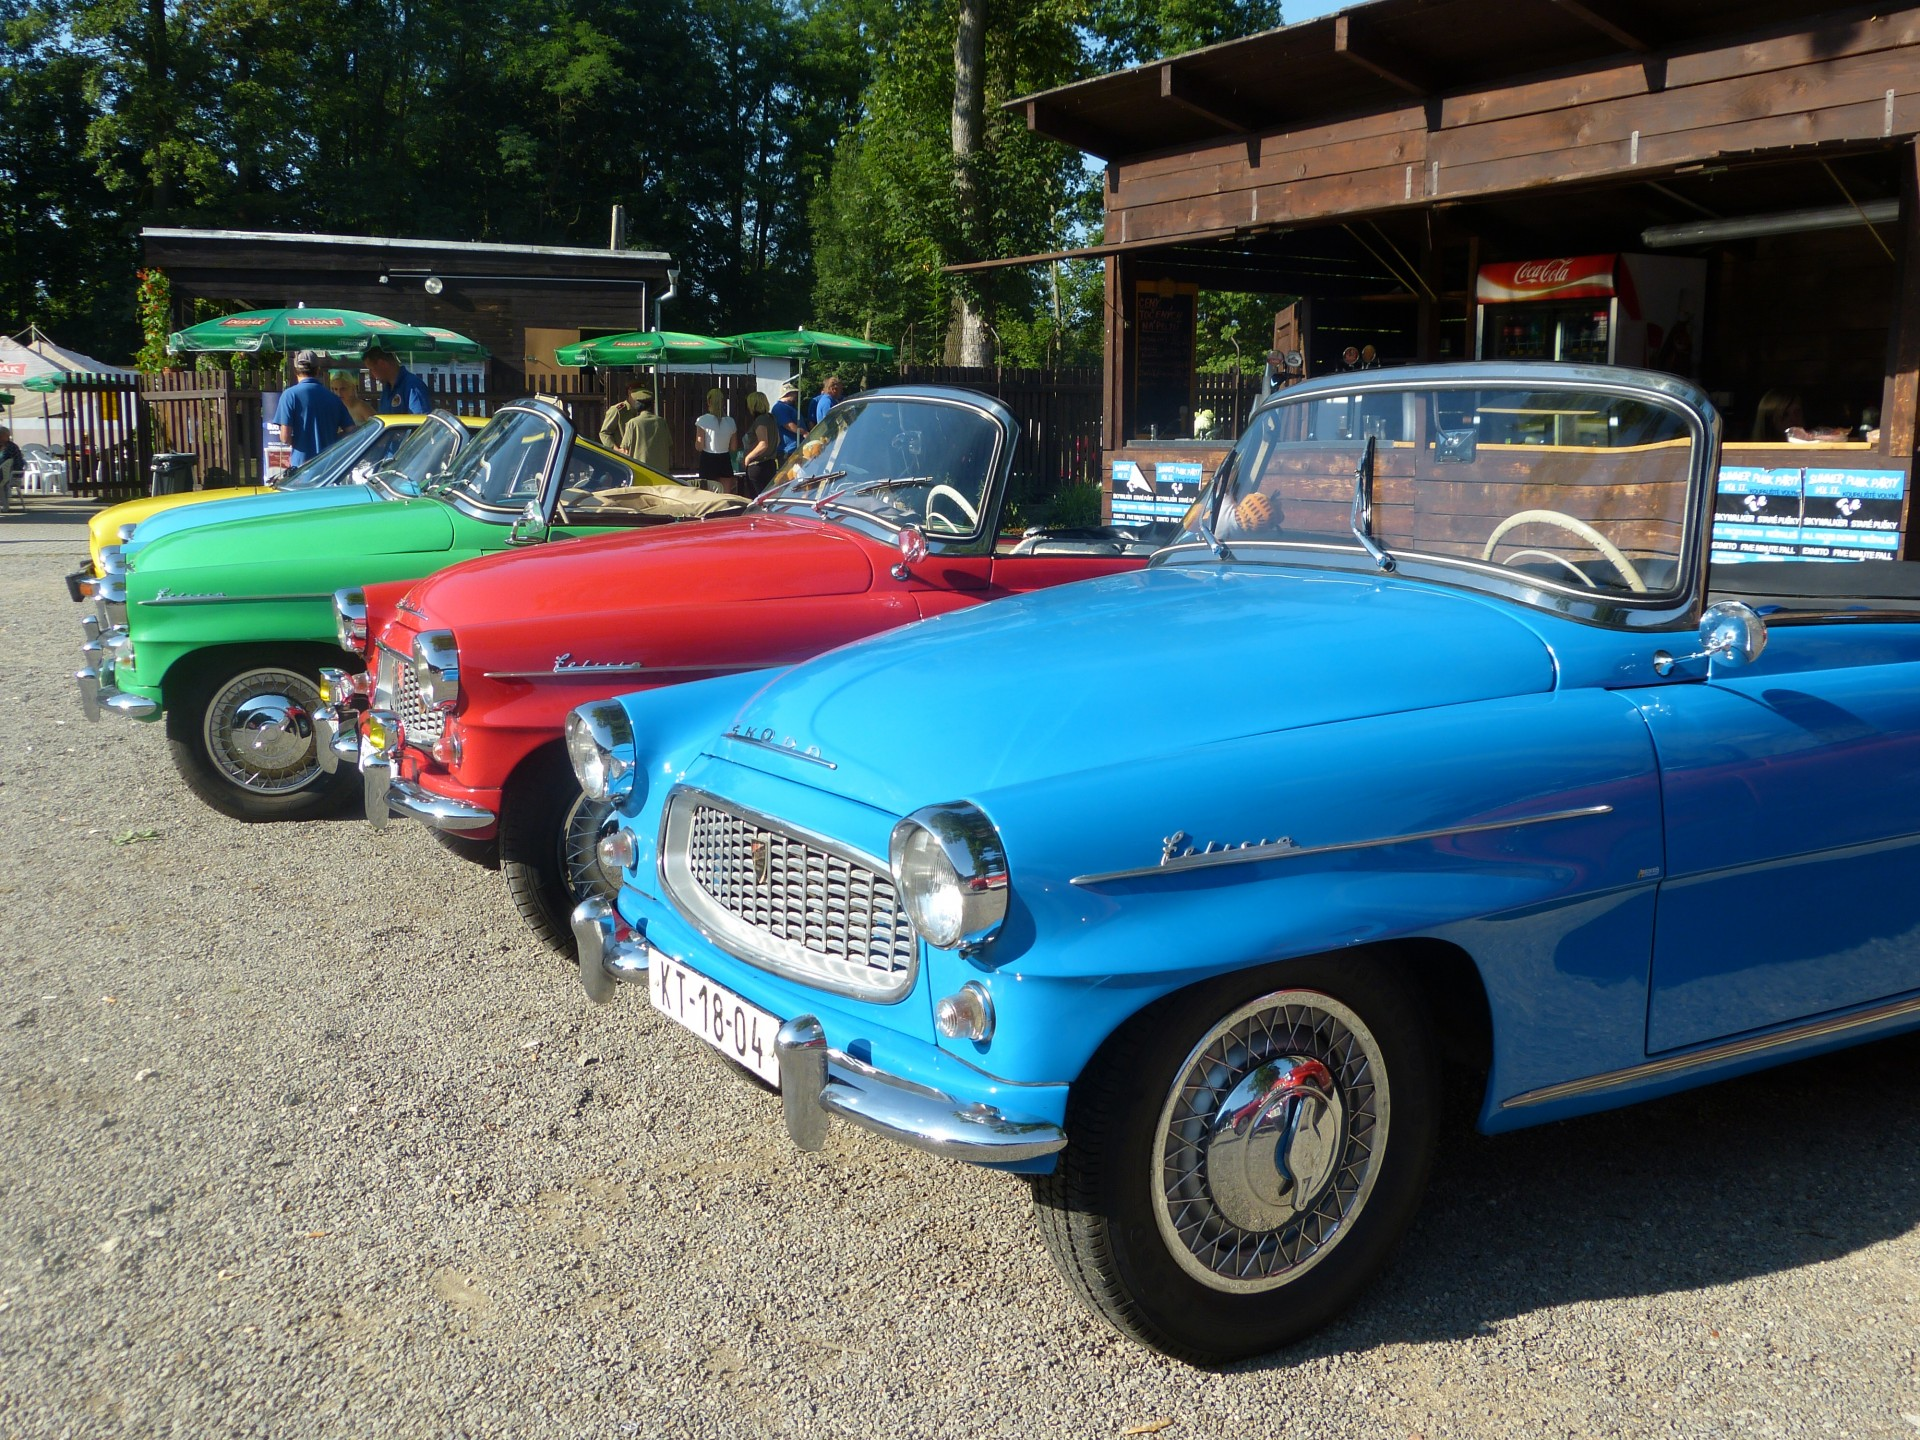
\includegraphics[width=0.3\textwidth]{old-cars.jpg}
	\end{center}

\end{frame}


\begin{frame}{Eksempler på klasser}
	\begin{itemize}
		\item Bil: \\
			Attributes: antal døre, producent, model\\
			Metoder: dyt(), stop(), start()
		\item Person: \\
			Attributes: navn, alder, forældre (Person)\\
			Metoder: hils(), skift\_navn(), løb()
	\end{itemize}
\end{frame}


\begin{frame}[fragile]{Har vi allerede brugt objekter?}
	\pause
	Vi har fx set et filobjekt:
	\begin{lstlisting}[style=python]
f = open("min_fil.txt", "w")
f.write("Lær python!!!\n")
f.write("IMADA SDU")
f.close()
	\end{lstlisting}
	Her bruger vi metoderne \texttt{write()} og \texttt{close()} på vores filobjekt.\\
\end{frame}


\begin{frame}[fragile]{Har vi allerede brugt objekter?}
		Filobjektet har også attributes fx:
	\begin{itemize}
		\item name: Navnet på filen (string)
		\item closed: Er filen lukket eller ej (boolean)
		\item mode: Hvordan er filen blivet åbnet (string)
	\end{itemize}
	\begin{columns}
		\column{0.5\textwidth}
		\begin{lstlisting}[style=python]
f = open("min_fil.txt", "w")
print(f.name)
print(f.closed)
print(f.mode)
f.close()
		\end{lstlisting}
		\column{0.3\textwidth}
		\begin{lstlisting}[style=python]
min_fil.txt
False
w
		\end{lstlisting}
	\end{columns}
\end{frame}

\section{Klasser og objekter i python}


\begin{frame}[fragile]{Definition af klasse}
	En klasse defineres på følgende vis:
		\begin{lstlisting}[style=python]
class Person:
	def __init__(self, name, age):
		self.name = name
		self.age = age
	\end{lstlisting}
	\texttt{\_\_init\_\_} er en speciel metode som bliver kaldt når et nyt objekt skal laves og kaldes for en \textit{constructor} metode. Denne metode skal have \texttt{self} som første parameter. Dette er en reference til objektet selv og bruges til at få adgang til objektets attributes.
\end{frame}

\begin{frame}[fragile]{Initialisering}
	Et nyt objekt kan nu laves, ved at :
		\begin{lstlisting}[style=python]
person1 = Person("Bamse", 25)
person2 = Person("Ruth", 78)
	\end{lstlisting}
	Og attributter kan tilgås vha. \texttt{.}-operatoren:
	\begin{lstlisting}[style=python]
print("person1:", person1.name, person1.age)
print("person2:", person2.name, person2.age)
	\end{lstlisting}
	Output:
	\begin{lstlisting}[style=python]
person1: Bamse 25
person2: Ruth 78
	\end{lstlisting}
\end{frame}

\begin{frame}{Hvor kan de bruges?}
	Objekter kan bruges alle steder hvor I er vant til at bruge variabler, f.eks.
	\begin{itemize}
		\item Som parameter til en funktion.
		\item Som en attribut i et andet objekt.
		\item Som returværdi fra en funktion.
	\end{itemize}
\end{frame}

\begin{frame}[fragile]{Eksempel}
	Lad os lave en klasse som gemmer et klokkeslæt:
		\begin{lstlisting}[style=python]
class Time:
	def __init__(self, h, m, s):
		self.hours = h
		self.mins = m
		self.secs = s
	\end{lstlisting}
	\pause
	Vi kan lave en funktion som printer tiden:
	\begin{lstlisting}[style=python]
def print_time(t):
	print("%02d:%02d:%02d" % (t.hours, t.mins, t.secs))
	\end{lstlisting}
\end{frame}

\begin{frame}[fragile]{Eksempel}
Lad os teste det:
\begin{columns}
	\column{0.4\textwidth}
	\begin{lstlisting}[style=python]
t = Time(2, 3, 23)
print_time(t)
	\end{lstlisting}
	\column{0.4\textwidth}
	\begin{lstlisting}[style=python]
02:03:23
	\end{lstlisting}
\end{columns}
\end{frame}




\section{Metoder}



\begin{frame}[fragile]{Hvad er det nye?}
Måske undrer I jer over, hvorfor man skulle bruge objekter, når man kunne gøre det samme med et dictionary:

\begin{lstlisting}[style=python]
def make_time(h, m, s):
  return {"hours": h, 
          "mins": m, 
          "secs": s}

def print_time(t):
  print("%02d:%02d:%02d" % (t["hours"], t["mins"], t["secs"]))

t = make_time(13,37,42)
print_time(t)
\end{lstlisting}
\end{frame}



\begin{frame}[fragile]{Hvad er det nye?}
Et problem kunne være hvis man ikke giver funktionen det rigtige:
\begin{columns}
\column{0.4\textwidth}
\begin{lstlisting}[style=python]
print_time("hej")
\end{lstlisting}
\pause
\column{0.45\textwidth}
\begin{lstlisting}[style=python]
Traceback (most recent...
File "test.py", line 6...
print_time("hej")
File "test.py", line 2...
print("%02d:%02d:%02d"...
TypeError: string indices must be integers
\end{lstlisting}
\end{columns}
\end{frame}

\begin{frame}[fragile]{Hvad er det nye?}
Vi kan løse det med metoder. Metoder er funktioner der tilhører objekter. Metoder skrives som en del af en klassedefinition.
\begin{lstlisting}[style=python]
class Time:
  ...

  def print_time(self):
    print("%02d:%02d:%02d" % (self.hours, self.mins, self.secs))
\end{lstlisting}
\pause
Vi har flyttet \textit{ansvaret} for at printe, til objektet selv.

\textbf{HUSK} metoder skal altid have \texttt{self} som første argument!

Desuden må ens metode ikke hedde det samme som en attribut. (f.eks. "sekunder" i dette tilfælde)
\end{frame}

\begin{frame}[fragile]{Hvad er det nye?}
Når man skal bruge metoden bruger man punktum.
\begin{columns}
\column{0.4\textwidth}
\begin{lstlisting}[style=python]
...
t = Time(13,37,42)
t.print_time()
\end{lstlisting}
\pause
\column{0.4\textwidth}
\begin{lstlisting}[style=python]
13:37:42
\end{lstlisting}
\end{columns}
\pause
Som I kan se, kan man nu ikke komme til at kalde funktionen forkert.
\end{frame}


\begin{frame}[fragile]{Tiden går}
Vi kan også ændre på et objekts værdier i en metode.
\begin{lstlisting}[style=python]
class Time:
  ...
  def wait(self, sekunder):
	  self.secs += sekunder
	  
	  self.mins += self.secs // 60
	  self.secs = self.secs % 60
	  
	  self.hours += self.mins // 60
	  self.mins = self.mins % 60
	  
	  self.hours = self.hours % 24
\end{lstlisting}
\end{frame}


\begin{frame}[fragile]{Tiden går}
Nu kan vi se, hvordan tiden går:
\begin{columns}
\column{0.4\textwidth}
\begin{lstlisting}[style=python]
...
t = Time(13,37,42)
t.print_time()
t.wait(59)
t.print_time()
\end{lstlisting}
\pause
\column{0.4\textwidth}
\begin{lstlisting}[style=python]
13:37:42
13:38:41
\end{lstlisting}
\end{columns}
\end{frame}

\begin{frame}[fragile]{Eksempel}
Husk stadig, at variabel navne er referencer til objekter, så et objekt kan blive ændret "et andet sted fra".
\begin{columns}
	\column{0.4\textwidth}
	\begin{lstlisting}[style=python]
t1 = Time(1, 2, 3)
t2 = t1
t2.print_time()
t1.wait(1)
t2.print_time()
	\end{lstlisting}
	\column{0.4\textwidth}
	\begin{lstlisting}[style=python]
01:01:01
01:01:02
	\end{lstlisting}
\end{columns}
\end{frame}


\section{Static methods}


\begin{frame}[fragile]{Static methods}
Nogle gange vil man gerne associere bestemte funktioner med en bestemt klasse, uden at de er knyttet til et specifikt objekt. I de tilfælde kan man lave static methods.

\pause
I vores tidseksempel kunne det være man vil have en funktion der altid kan give os frokost tidspunktet 12:00:00. Det kunne se således ud:
\begin{columns}
	\column{0.4\textwidth}
	\begin{lstlisting}[style=python]
class Time:
  ...
  
  def noon():
    return Time(12,0,0)

t = Time.noon()
t.print_time()
	\end{lstlisting}
	
	\column{0.4\textwidth}
	\begin{lstlisting}[style=python]
12:00:00
	\end{lstlisting}
\end{columns}

\pause
Forskellen er at vi ikke har \texttt{self} som parameter, og at vi bruger klassenavnet til at få adgang til funktionen.

\end{frame}

\begin{frame}[fragile]{Static methods}
Et andet eksempel kunne være at vi ville have en funktion der kan sammenligne to personer, og svare på om den ene er ældre end den anden.

\begin{columns}
	\column{0.52\textwidth}
	\begin{lstlisting}[style=python]
class Person:
	...
	
	def older(p1, p2):
		return p1.age > p2.age

jens = Person("Jens", 35)
peter = Person("Peter", 27)
print(Person.older(jens, peter))
	\end{lstlisting}
	\pause
	\column{0.3\textwidth}
	\begin{lstlisting}[style=python]
True
	\end{lstlisting}
\end{columns}

\end{frame}


\section{Magic methods m.m.}



\begin{frame}[fragile]{Specielle metoder}
Vores tidligere metode \texttt{print\_time} hjælper os med at printe tiden, men hvad nu hvis man gerne vil printe den sammen med noget andet?
\begin{lstlisting}[style=python]
Klokken er 13:37:42 lige nu.
\end{lstlisting}
\pause
Og hvad sker der egentlig hvis vi printer tid, lige nu?
\begin{columns}
\column{0.4\textwidth}
\begin{lstlisting}[style=python]
...
t = Time(13,37,42)
print(t)
\end{lstlisting}
\pause
\column{0.4\textwidth}
\begin{lstlisting}[style=python]
<__main__.Time object at 0x02B11890>
\end{lstlisting}
\end{columns}
\end{frame}


\begin{frame}[fragile]{Specielle metoder}
Der findes en masse specielle metoder, nogle gange kaldet magic methods, som bliver kaldt på nogle bestemte tidspunkter og har nogle bestemte krav. Man kan kende dem på at de har to underscores både før og efter navnet, så I har allerede set én, \texttt{\_\_init\_\_}, som kaldes for en constructor funktion.

En anden meget brugt af disse er \texttt{\_\_repr\_\_} som skal returnere en streng, og meningen er at det er sådan objektet repræsenteres som en streng.
\begin{lstlisting}[style=python]
class Time
  ...
  def __repr__(self):
    return "%02d:%02d:%02d" % (self.hours, self.mins, self.secs)
\end{lstlisting}
\end{frame}

\begin{frame}[fragile]{Specielle metoder}
Så nu behøver vi ikke \texttt{print\_time} metoden længere, og vi har fået endnu mere fleksibilitet med.
\begin{columns}
\column{0.4\textwidth}
\begin{lstlisting}[style=python]
...
t = Time(13,37,42)
print(t)
print("Klokken er", 
      t, "lige nu.")
\end{lstlisting}
\pause
\column{0.45\textwidth}
\begin{lstlisting}[style=python]
13:37:42
Klokken er 13:37:42 lige nu.
\end{lstlisting}
\end{columns}
\end{frame}

\begin{frame}[fragile]{Specielle metoder}
Der findes rigtig mange flere, men dem må I selv læse mere om på nettet. Bare husk at de kan række dybt ind i Pythons maskineri, så brug dem med omtanke.
\end{frame}
%\section{Metoder}
%
%
%\section{Nedarvning}




\end{document}